
\subsection{3D Rate Results}
\begin{frame}
	\frametitle{3D Multi Pad}
	\begin{itemize}
		\item \SI{500}{\micro\meter} thick poly-crystalline diamond sensor
		\item 25 3D cells ganged together into a single readout (quasi-pad)
	\end{itemize}
	\begin{figure}
		\centering
		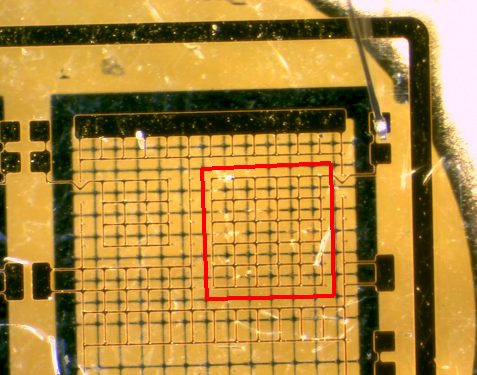
\includegraphics[width=6cm]{3DPhoto}
	\end{figure}
\end{frame}
% ============================ new frame ==========================================>
\begin{frame}
	\frametitle{3D Multi Pad - Signal Maps}
	\begin{figure}
		\centering
		\begin{subfigure}[t]{0.45\textwidth}
			\centering
			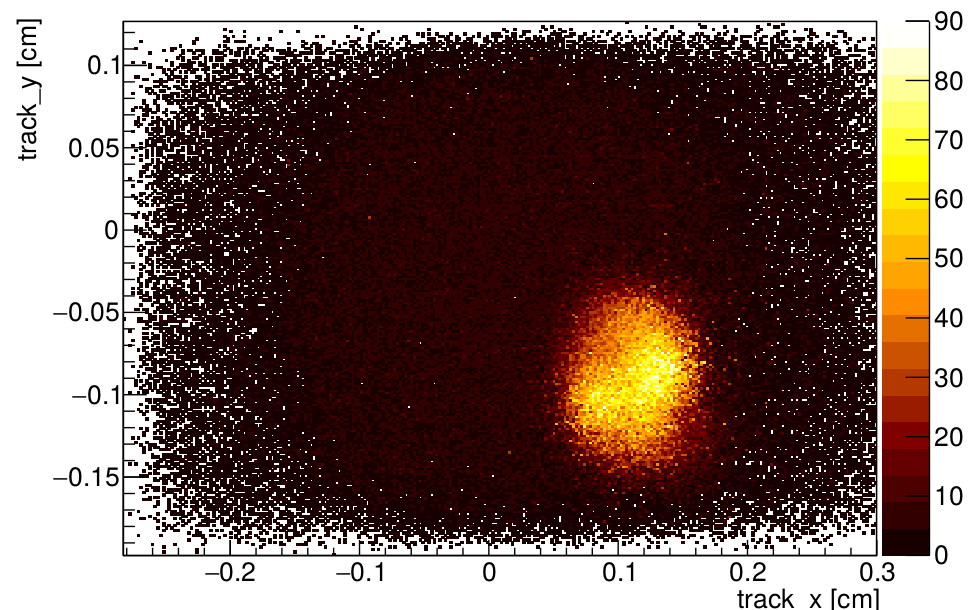
\includegraphics[width=5cm]{3DMap}
% 			\caption{blue: Diamond peak. Orange and black: Graphitic material}
		\end{subfigure}
		\begin{subfigure}[t]{0.45\textwidth}
			\centering
			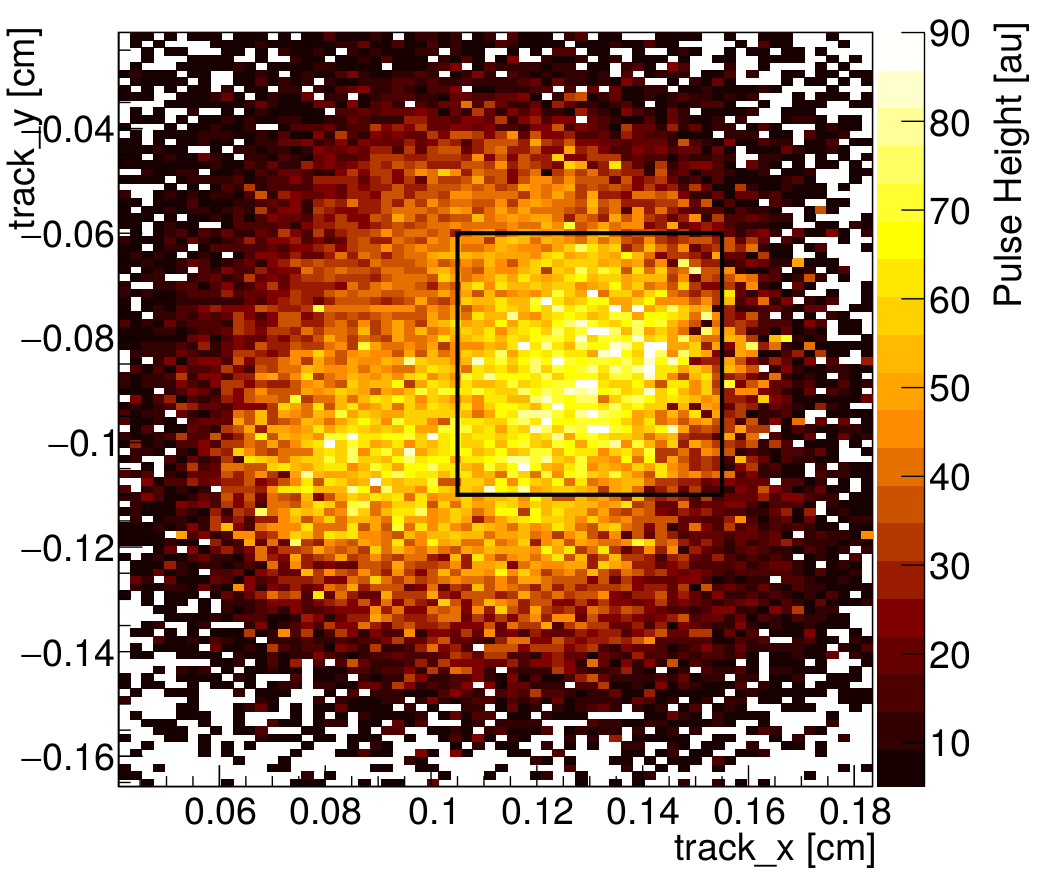
\includegraphics[height=5cm]{3DMapZoom}
% 			\caption{square and hexagonal bias patterns (red) and readout channels (blue).}
		\end{subfigure}
	\end{figure}
\end{frame}
% ============================ new frame ==========================================>
\begin{frame}
	\frametitle{3D Multi Pad - Pulse Height}
	\begin{figure}
		\centering
		\begin{subfigure}[t]{0.45\textwidth}
			\centering
			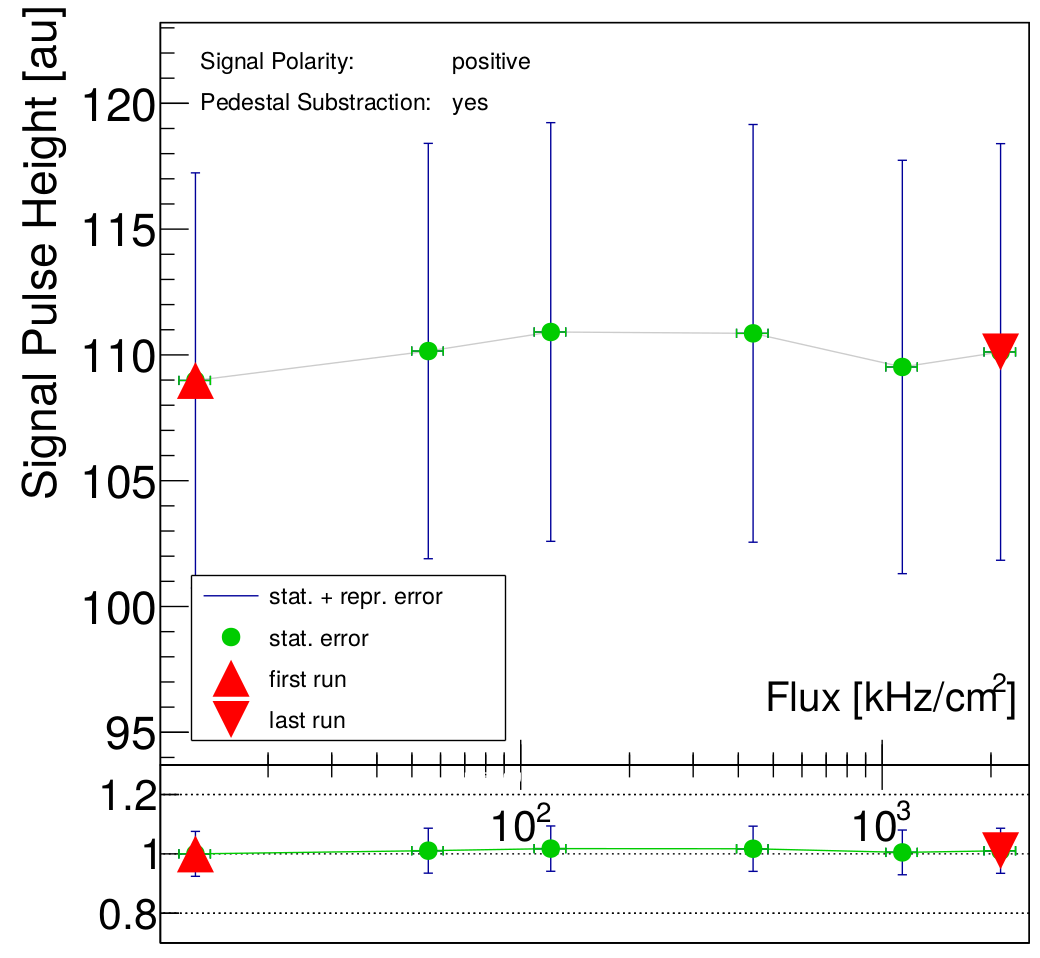
\includegraphics[height=5cm]{SiDPH}
			\caption{\SI{100}{\micro\meter} silicon diode}
		\end{subfigure}
		\begin{subfigure}[t]{0.45\textwidth}
			\centering
			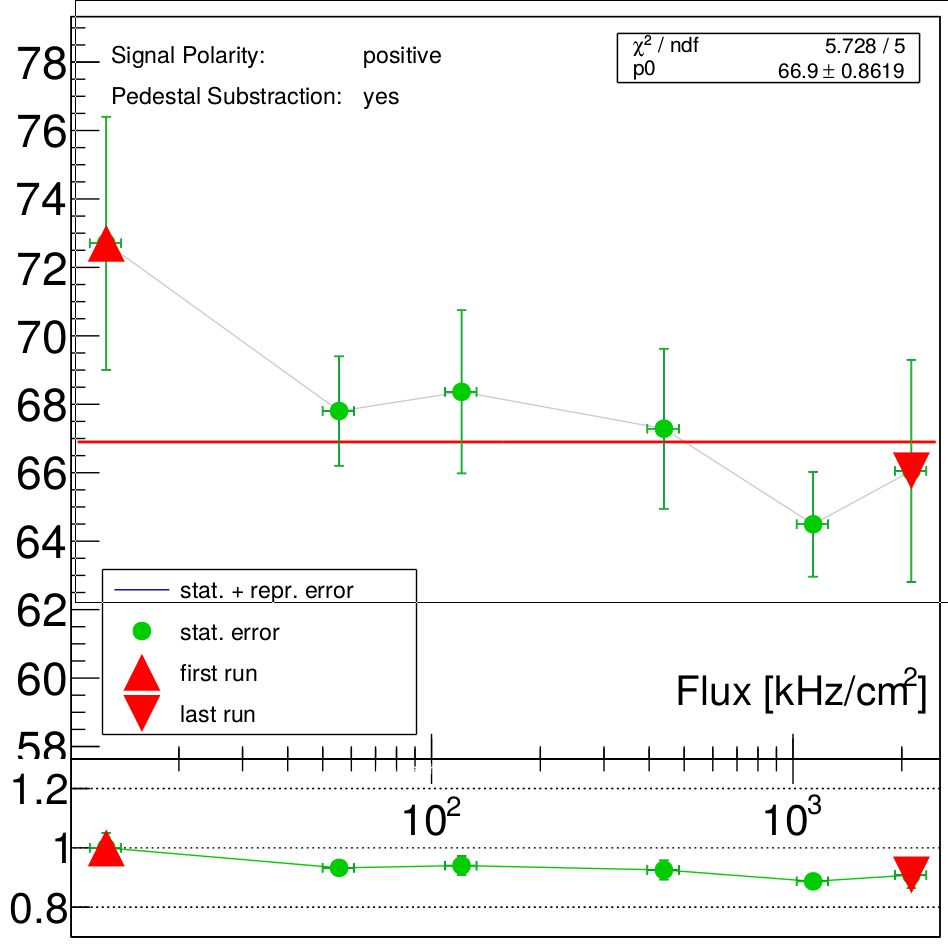
\includegraphics[height=5cm]{3DPH}
			\caption{\SI{500}{\micro\meter} poly-crystalline diamond}
		\end{subfigure}
	\end{figure}
	\begin{itemize}
		\item pulse height in diamond three times less than expected!
		\begin{itemize}
			\item under investigation
		\end{itemize}
	\end{itemize}

\end{frame}